\documentclass{article}
\usepackage[top=1in,bottom=1in,left=1in,right=1in]{geometry}
\usepackage{listings}
\usepackage{hyperref}
\usepackage{color}
\usepackage[pdftex]{graphicx}
\usepackage{xspace}


\title{Models of FMDV in a Herd of Cattle}
\author{Drew Dolgert}
\date{\today}

\begin{document}
\maketitle
\abstract{There is significant data on the progress of FMDV within individual
cattle. This data describes both the progress of the disease and its variability
among individuals according to various effects. Obtaining multiple samples of
similar data for herds of infected cattle is impractical or inhumane, so
models extend understanding at an individual level to a herd level. This article
examines a family of models for FMDV progress within a herd in order to
understand how both the average progress of disease and an estimate of its
variability.}

\section{Introduction}
Focus on a putative herd of beef cattle of the same breed and similar life stage.
Build several models of varying complexity.

This will work with compartmental models in continuous time.
We will look at a series of models. A model is defined as a set
of states, transitions which modify the states, and rates for those
transitions. For each variant of a model, look at which of these
three is varied.

There are a series of types of models.
\begin{enumerate}
  \item Individual---weight, age progression, gains
  \item Individual Disease Pathology
  \begin{enumerate}
    \item Compartmental states
    \item Hazard rates
    \item Frailties
  \end{enumerate}
  \item Single Herd
  \begin{enumerate}
    \item Contact rate and structure
    \begin{enumerate}
      \item Well-mixed
      \item Simulated from statistical model
    \end{enumerate}
    \item Disease progression given contact
  \end{enumerate}
  \item Feedlot
  \begin{enumerate}
    \item Pens
    \item Hospital pens
    \item Demographics and incoming/slaughter
    \item Agents such as riders, wildlife, 4H clubs
    \item Background transport, airborne or unidentified
  \end{enumerate}
  \item Detection
  \begin{enumerate}
    \item Clinical states
    \item Conditions, meaning percent diseased before detection
  \end{enumerate}
  \item Intervention
  \begin{enumerate}
    \item Conferred immunity
    \item Vaccination/culling team work rates
  \end{enumerate}
\end{enumerate}

\section{Stochastic Compartmental Models in Continuous Time}
This section explains how to define the kind of model used
in this article. It doesn't describe how simulation is done.

\begin{figure}
\centerline{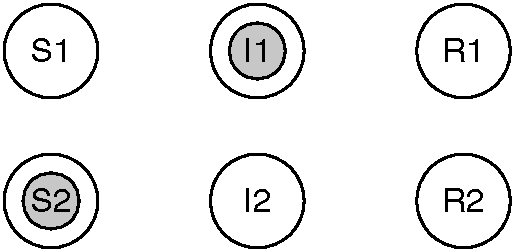
\includegraphics[width=4cm]{place_with_tokens}}
\caption{Each circle is a place. A token on I1 is a representation
of individual 1 being infectious. A token on S2 shows individual 2
is susceptible.\label{fig:placewithtokens}}
\end{figure}%
Think of an individual which passes through a series of states.
It might seem obvious to assign to that individual a category,
latent, infectious, or recovered. Instead, think of the individual
as a piece on a checkerboard. Its location on the board indicates
the state of the individual. The checker is called a Token, and
the location is called a Place. The Places might be named
individual-1-is-latent, individual-1-is-infected, and individual-1-is-recovered.
Were there a second individual, it could be represented by a second
token on a second set of places,
individual-2-is-latent, individual-2-is-infected, and individual-2-is-recovered,
as shown in Fig.~\ref{fig:placewithtokens}.
There are certain occasions, when using exponenentially-distributed
transitions, that the Places for both individuals could be combined,
putting both tokens on an any-individual-is-latent place.
The state of the system, at any time, is defined by the
combination of which tokens are at which places, and by the
enabling times of transitions.

\begin{figure}
\centerline{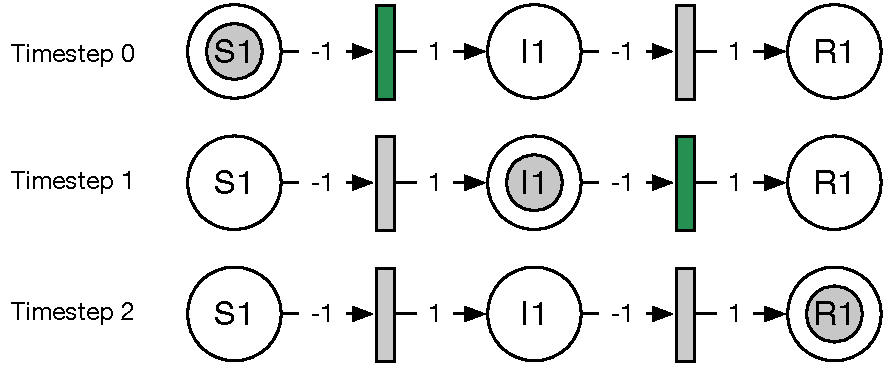
\includegraphics[width=5cm]{move_tokens_sir}}
\caption{Transitions move tokens among places. Green transitions
are enabled because there are tokens at their input places.
Each row represents a step in the simulation. After the infection
transition fires, the token moves, enabling the recovery transition
and disabling the infection transition. After the next step,
no transitions are enabled.\label{fig:movetokenssir}}
\end{figure}%
Transitions define the dynamics of the system, how and when Tokens
move among Places. Associated with each transition is a
conditional probability distribution with a continuous distribution.
For instance, an animal cannot recover until it has become infected,
so the distribution for recovery depends upon first being infected,
corresponding to a Token on the infected place. The arrival
of a token at the infected place, from some previous transition,
is said to enable the recovery transition. Once enabled, that
transition will fire at some later time determined by the
continuous distribution over times-since-enabling.
Fig.~\ref{fig:movetokenssir} shows a sequence of transitions
firing, moving a token to different Places, changing system state.

\begin{figure}
\centerline{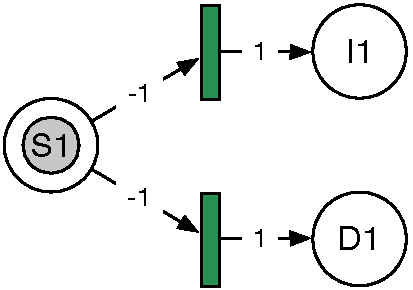
\includegraphics[width=3cm]{censor_gspn}}
\caption{This represents what medical trials call right-censoring.
The possible transition to Place D censors data about the rate
of transitions to Place I, for infections. For instance,
a cattlebeast could be sent to slaughter before infection
could occur.\label{fig:censorgspn}}
\end{figure}%A single transition can depend on the presence of more than one
input token and can move more than one token when it fires.
Because of this complexity, transitions are represented not
with arrows but with rectangles on diagrams. Drawing separate
transitions on diagrams is a good reminder of a distinction
familiar to those who work with medical studies and censoring. Given
a state where two different transitions can fire, each
disabling the other, each transition has its own distribution
of times at which it fires. This is shown in
Fig.~\ref{fig:censorgspn}. These two, together, determine
a third distribution, the waiting time distribution of
how long the token remains in the Place since its arrival
at that Place. If an infected animal can either recover
or die, then its waiting time in the infected state is
determined by the transition distributions to the recovered
and dead states. Speaking of an ``infection interval'' can,
in the presence of competing transitions, be unclear.



\section{FMDV progress within an individual}
\begin{figure}
\centerline{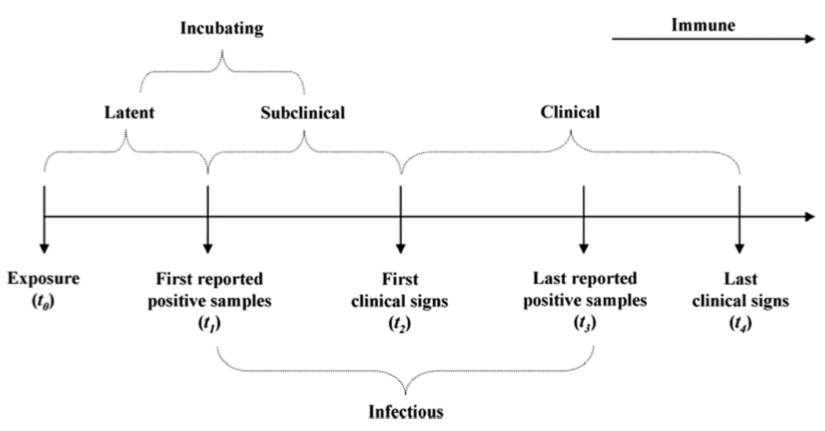
\includegraphics[width=9cm]{mardones_states}}
\caption{Time points for observations from Mardones et al.\cite{Mardones2010}.
Each observation is a transition to a new state.\label{fig:mardones_states}}
\end{figure}
\begin{figure}
\centerline{\begin{tabular}{lllll}
\hline
FMD stage & time interval [days] & State Transition & Poisson & Distribution \\ \hline
Latent &  $t_1-t_0$ & $(I,0,0)$--$(I,1,0)$ & 3.59 & Weibull ($\alpha=1.782$, $\beta=3.974$) \\
Subclinical & $t_2-t_1$ & $(I,1,0)$--$(I,1,1)$ & 2.04 & Gamma ($\alpha=1.222$, $\beta=1.672$) \\
Incubation & $t_2-t_0$ & $(I,0,0)$--$(I,1,1)$ & 5.9 & Log logistic ($\gamma=0$, $\beta=5.3$, $\alpha=4.02$) \\
Infectious &  $t_3-t_1$ & $(I,1,0)$--$(R,0,1)$ & 4.39 & Gamma ($\alpha=3.969$, $\beta=1.107$) \\
Clinical Recovery & $t_4-t_2$ & $(I,1,1)$--$(R,0,0)$ & NA & NA
\end{tabular}}
\caption{From ``FMDV serotype O infection in domestic animals,''\label{fig:compartments}}
\end{figure}%
\begin{figure}
\centerline{\begin{tabular}{llll}
\hline
Viral Load & Infectiousness & Clinical Sign & Seen in FMDV \\ \hline
Susceptible & 0 & 0 & Susceptible state \\
Infected & 0 & 0 & Latent state \\
Infected & 0 & 1 & not seen \\
Infected & 1 & 0 & Infectious, sub-clinical \\
Infected & 1 & 1 & Infectious, clinical \\
Recovered & 0 & 1 & Recovered, clinical \\
Recovered & 0 & 0 & Recovered, sub-clinical
\end{tabular}}
\caption{This lists all possible states of an individual
with these three separate measurable traits. Listing all possible
states is a first step towards choosing how to represent
the states and transitions among those states.\label{fig:allstates}}
\end{figure}%
In an epidemiological context, a compartmental model reduces
the pathology of FMDV to whether inoculation and recovery have happened,
whether the animal is infectious, and whether the animal shows
visible clinical signs of infection. These differentiate among
viral load within the animal, shedding of virus, and visible
immune response. They create a table of possible states, shown
in Fig.~\ref{fig:allstates},
only some of which are witnessed for the progression of FMDV.

For continuous-time models, no two transitions are simultaneous,
so a chart of all possible transitions includes a transition
for a change in any one of the three traits. For instance,
there may be a transition from $(I,0,0)$, which represents
an infected state with no infectiousness or clinical sign,
to $(I,0,1)$ or to $(I,1,0)$ but no direct transition to $(I,1,1)$,
a state which is both infectious and clinical. The chart
of possible transitions is shown in Fig.~blah.
It is colored according to states described by Mardones
et al.\ in a review paper.

That paper focuses on those transitions most important for
the progress of disease, as defined from five observation
points, exposure at $t_0$, first reported positive sample
at $t_1$, first clinical sign at $t_2$, last reported positive sample at $t_3$,
and last clinical sign at $t_4$. A diagram of this timeline is
in Fig.~\ref{fig:compartments}.
The observations are implicitly ordered in time, as 0 through 4,
although this is not guaranteed for other diseases where, for instance,
clinical sign might precede infectiousness.
From these are defined five transitions, shown in Fig.~\ref{fig:compartments}.
The transition from clinical back to subclinical is excluded,
presumably because it is both less important and without
significant data. Note also that the end of infectiousness
coincides with the end of infection in this model, eliding
the two possible states, $(I,0,1)$ and $(R,0,1)$, in the
general model.

Mardones et al.\ offer two different ways to specify
when clinical signs begin. One is an Incubation transition. The
other is two transitions in a row, through the latent and subclinical
stages. These alternatives express conditional dependency.
If clinical signs depend upon infectiousness, then the two-step
process is appropriate. If they are independent, then the incubation
period is the correct representation. A simulation using
the incubation period would not guarantee that
infection occurs before incubation, except insofar as
the transition rates encourage this ordering.
A stochastic compartmental model represents independent
processes, such as becoming clinical and becoming
infectious, as transitions which affect different substates
of the system, so the alternative dependencies become
alternative representations of the compartmental model,
shown in Fig.~\ref{fig:individual_gspn}.
For neither representation do the allowed transitions correspond
exactly to those suggested by the time-ordered compartments
shown in Mardones et al., but they both capture
the most important stages of FMDV.

\begin{figure}
\centerline{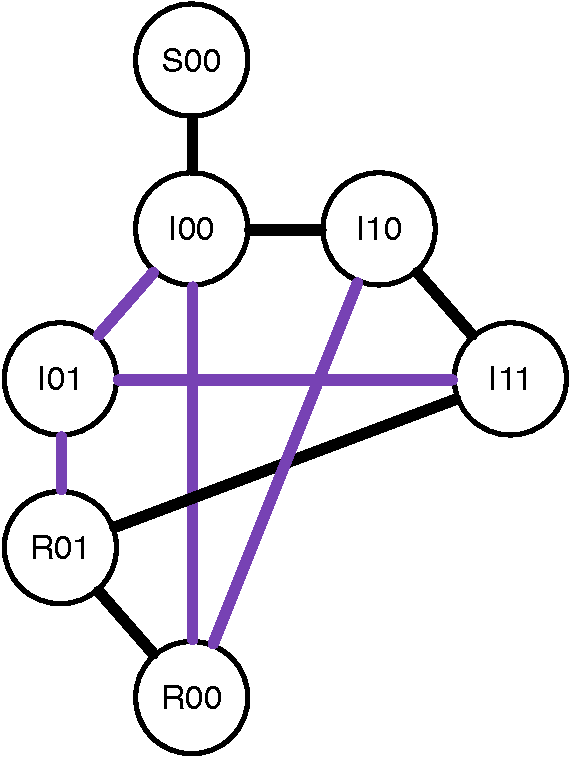
\includegraphics[width=4cm]{all_states}}
\caption{This shows all possible states for an individual.
The solid lines represent the abstract possibility for a transition
among neighboring states, in either direction from state to state.
Our model must be a subset of these
states and transitions. The ordering of events in Mardones et
al.\ suggests only the path colored black.\label{fig:all_states}}
\end{figure}
\begin{figure}
\centerline{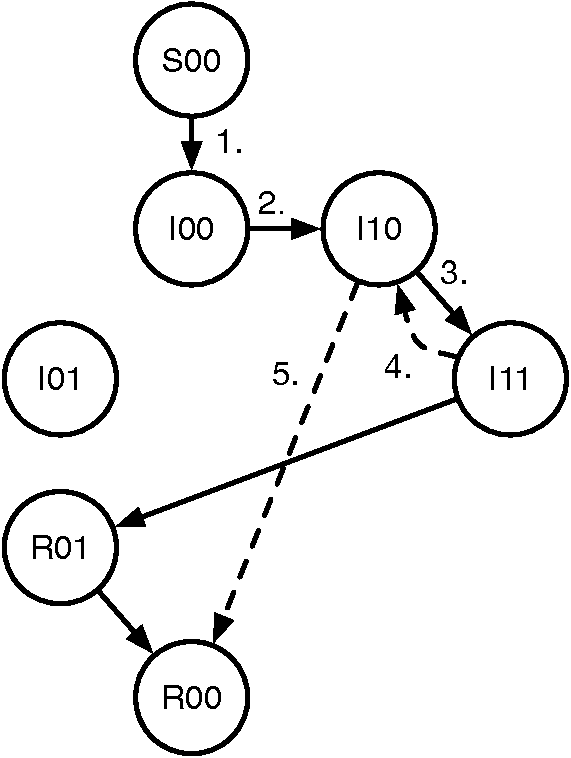
\includegraphics[width=4cm]{state_space_mardones}}
\caption{The Mardones paper suggests a time-ordered set of
states, shown with solid lines. It is not possible for an
animal to become clinical when it is not yet infectious.
If the times, $t_3$ and $t_4$ may be reordered, $t_4<t_3$,
so that clinical recovery can occur before recovery from
infection,
then the dotted line shows an allowed transition for which
the sequence of transitions is labeled.
The GSPN representations shown below will disallow the
transition labeled 4, but permitting it could be done,
as well.\label{fig:state_space_mardones}}
\end{figure}

\begin{figure}
\centerline{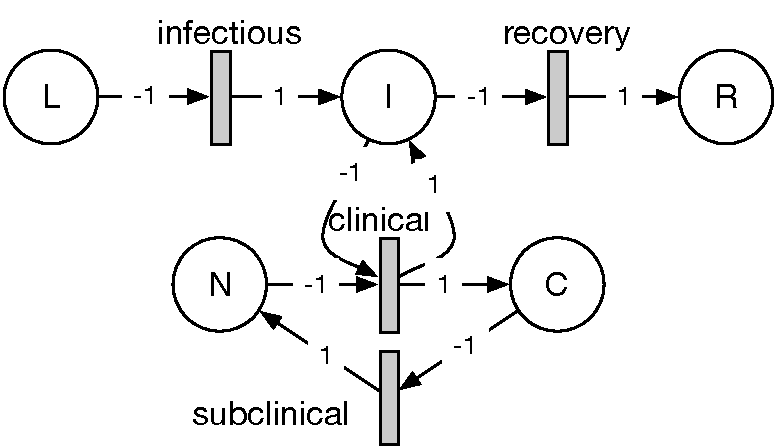
\includegraphics[width=6cm]{individual_gspn}}
\caption{The four compartmental states of an animal with FMDV
are represented by two categories, $(S,I,R)$ and $(N,C)$
where $N$ and $C$ represented not-clinical or clinical.
Computation proceeds by moving a token among $(S,I,R)$ and a
second token among $(N,C)$. Rectangles represent transitions,
which are enabled only when tokens are at all input edges to the
transition.\label{fig:individual_gspn}}
\end{figure}
\begin{figure}
\centerline{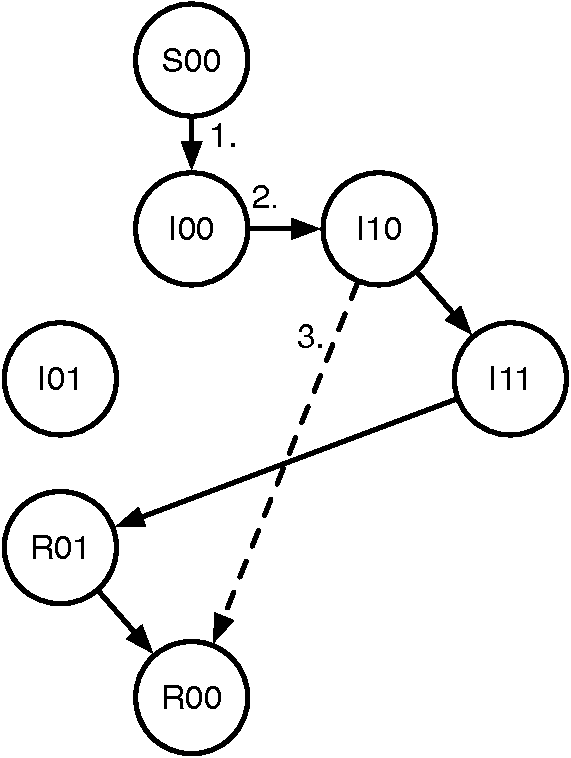
\includegraphics[width=4cm]{state_space_dependent}}
\caption{For the GSPN shown in Fig.~\ref{fig:individual_gspn},
the allowed set of transitions includes the possibility
of not traversing the state $(I,1,1)$ at any point. That is,
the animal will never be clinical if it recovers sooner
than it becomes clinical. This depends on the choice of
distributions for firing times.\label{fig:state_space_dependent}}
\end{figure}


\begin{figure}
\centerline{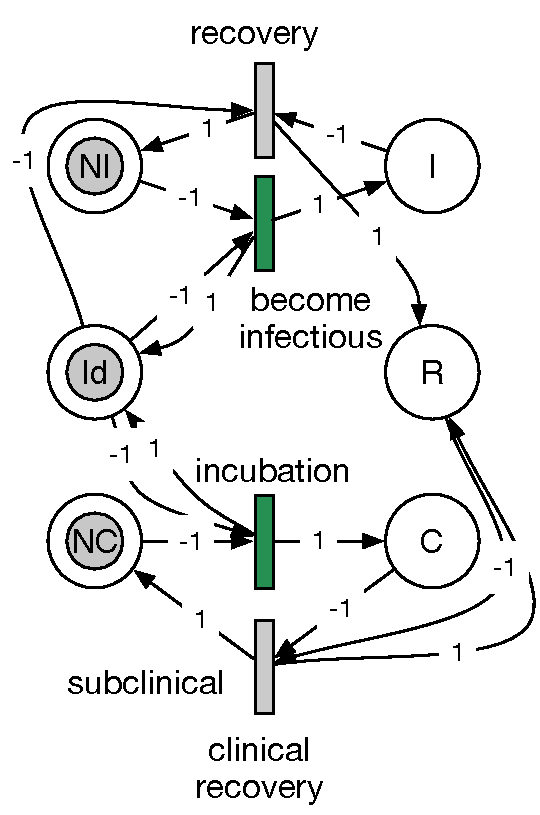
\includegraphics[width=4cm]{individual_indep_gspn}}
\caption{Here the transition to clinical is considered independent
of when the individual becomes infectious. The initial state of the
system consists of three tokens, one at Id, the infected state,
one at NI, the not-infectious state, and one at NC, the not-clinical
state. When tokens are located at the removed state, R, and the NI
and NC states, the disease has run its course in this individual.
\label{fig:individual_indep_gspn}}
\end{figure}
\begin{figure}
\centerline{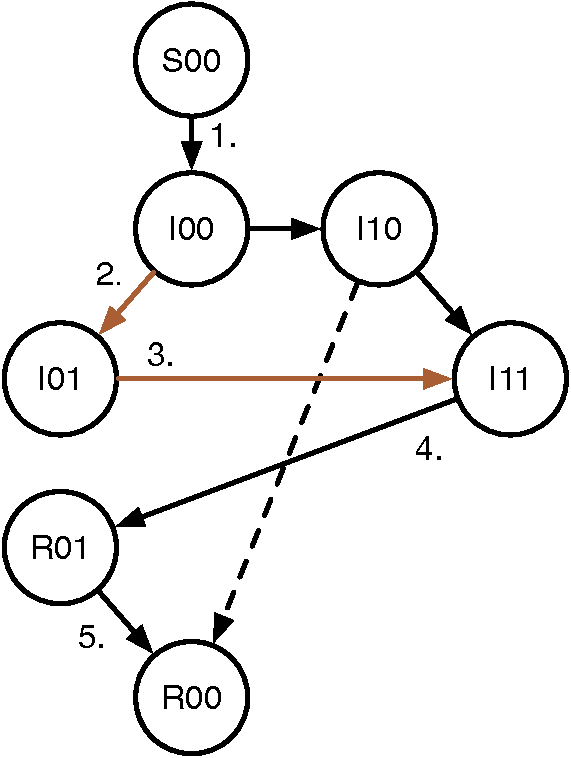
\includegraphics[width=4cm]{state_space_independent}}
\caption{The state space and transitions for Fig.~\ref{fig:individual_indep_gspn}
does include the possibility of becoming clinical before
becoming infectious, because the two transitions are simultaneous
and independent. That is shown with labels 2. and 3.
How often this state occurs is controlled by the shape
of the incubation distribution.\label{fig:state_space_independent}}
\end{figure}

\begin{figure}
\centerline{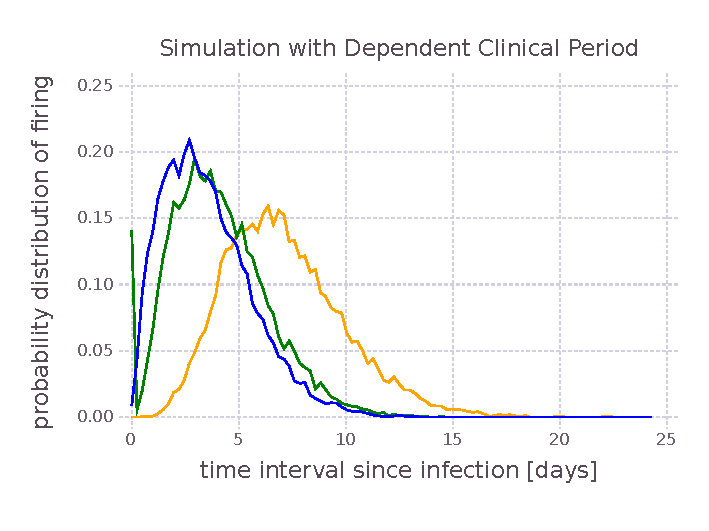
\includegraphics{SimulationwithDependentClinicalPeriod}}
\caption{This simulation first finds the time until
infectiousness begins and simulates start of clinical symptoms
from that time point.
Blue=infectious, Green=clinical, Orange=removed. The mass near
zero for clinical cases indicates simulations where the individual
entered the removed state before it could become clinical.
\label{fig:depclinicalindividual}}
\end{figure}
\begin{figure}
\centerline{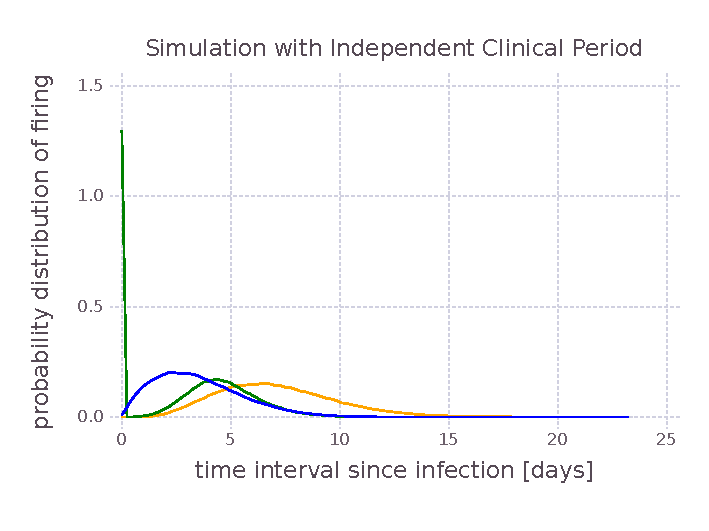
\includegraphics{SimulationwithIndependentClinicalPeriod}}
\caption{This simulation uses the Incubation distribution from
Mardones et al.\ in order to estimate the incubation period
independent from the beginning of the infectious period.
Blue=infectious, Green=clinical, Orange=removed. The mass near
zero for clinical cases indicates simulations where the individual
entered the removed state before it could become clinical.
\label{fig:indepclinicalindividual}}
\end{figure}
\begin{figure}
\centerline{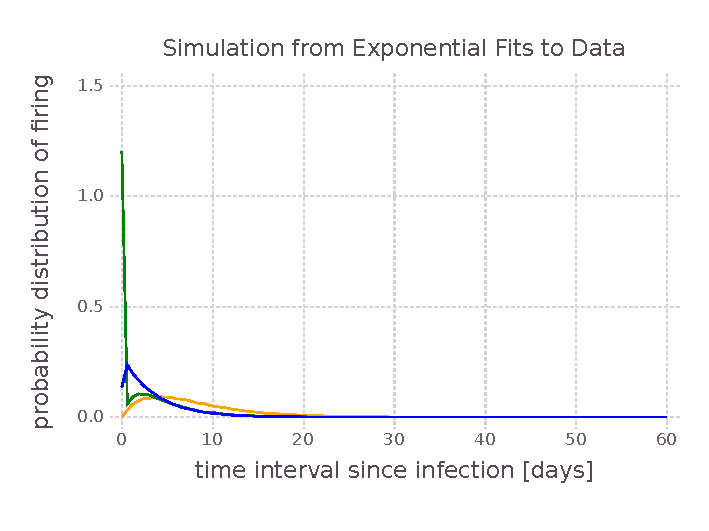
\includegraphics{SimulationfromExponentialFitstoData}}
\caption{Were the simulation to use exponential fits to observation
data, this would be the predicted distribution of infection,
clinical sign and recovery. The average times to each are the same
as those in the nonexponential fits, but the distribution of
times is much different.
\label{fig:individualexponential}}
\end{figure}
Simulations of both models show that, while average rates
are the same, the distribution
of times to infection or recovery can be quite different.
How much this matters depends on the application, which
here is prediction of prevalence within a herd.

\subsection{$R_0$ for Nonexponential Model}
$R_0$ is determined by the number of individuals a single
infected will infect. How do we compute $R_0$ given non-exponential
distributions? In this case, an individual in the
infectious state will either recover or infect others. Infecting
others is an exponential process with hazard $\beta S$, where
$S$ is the number of susceptibles. How long will the individual
remain infectious? Assume a constant rate of infection of others
over that time, which approximates the decreasing number of
susceptibles. Using $G(\tau)=1-F(\tau)$ as the survival,
\begin{equation}
  \int_0^\infty \beta S \tau G(\tau)d\tau
\end{equation}

\section{Herd Models}
Spread of infection within a herd of cattle is complicated.
Using a compartmental model built from the individual
models above distills complication into variation in
individual compartments and transitions, contact structure,
and infection rate given that contact structure.
How cattle fraternize in a field can be seen as a
time-dependent contact graph whose structure is 
distinct from the infection process which takes place
on that graph. For instance, if the shortest path between
two individuals in the graph is four individuals long, then
\emph{any\/} disease will require two latent periods
to travel from one individual to another.

\begin{itemize}
  \item Exponential or non-exponential individual model.
  \item Time-dependent contact hazard or frequency-dependent contact.
\end{itemize}

\bibliography{cattleherd}
\bibliographystyle{plain}
\end{document}
